\chapter{Trijunction of Majorana nanowires}

In this chapter we demonstrate that the coupling of three pairs of MBS in a trijuction is determined by the geometrical details of the central semiconducting cavity.
For certain geometrical configurations, a MBS pair couples resonantly with successive cavity states as in the so-called \textit{resonant trapping}, while in other cases the coupling is mediated by individual non-overlapping levels.

We simulate the pair coupling of three Majorana nanowires mediated by a semiconducting cavity using Kwant.
For each experiment, a pair of nanowires is set to host MBS in each sub band while the other nanowire is fully depleted.
We consider the strong coupling regime where there are no tunnel barriers between the cavity and the nanowires.
Furthermore, the phase difference between the selected nanowires is tuned such that the coupling is at a maximum.
\textit{The coupling energy of each pair is extracted as the value of the lowest non-zero eigenvalue with respect to the cavity chemical potential}.

\section{Quasi-one dimensional cavities}

\begin{figure}[h!]
\centering
  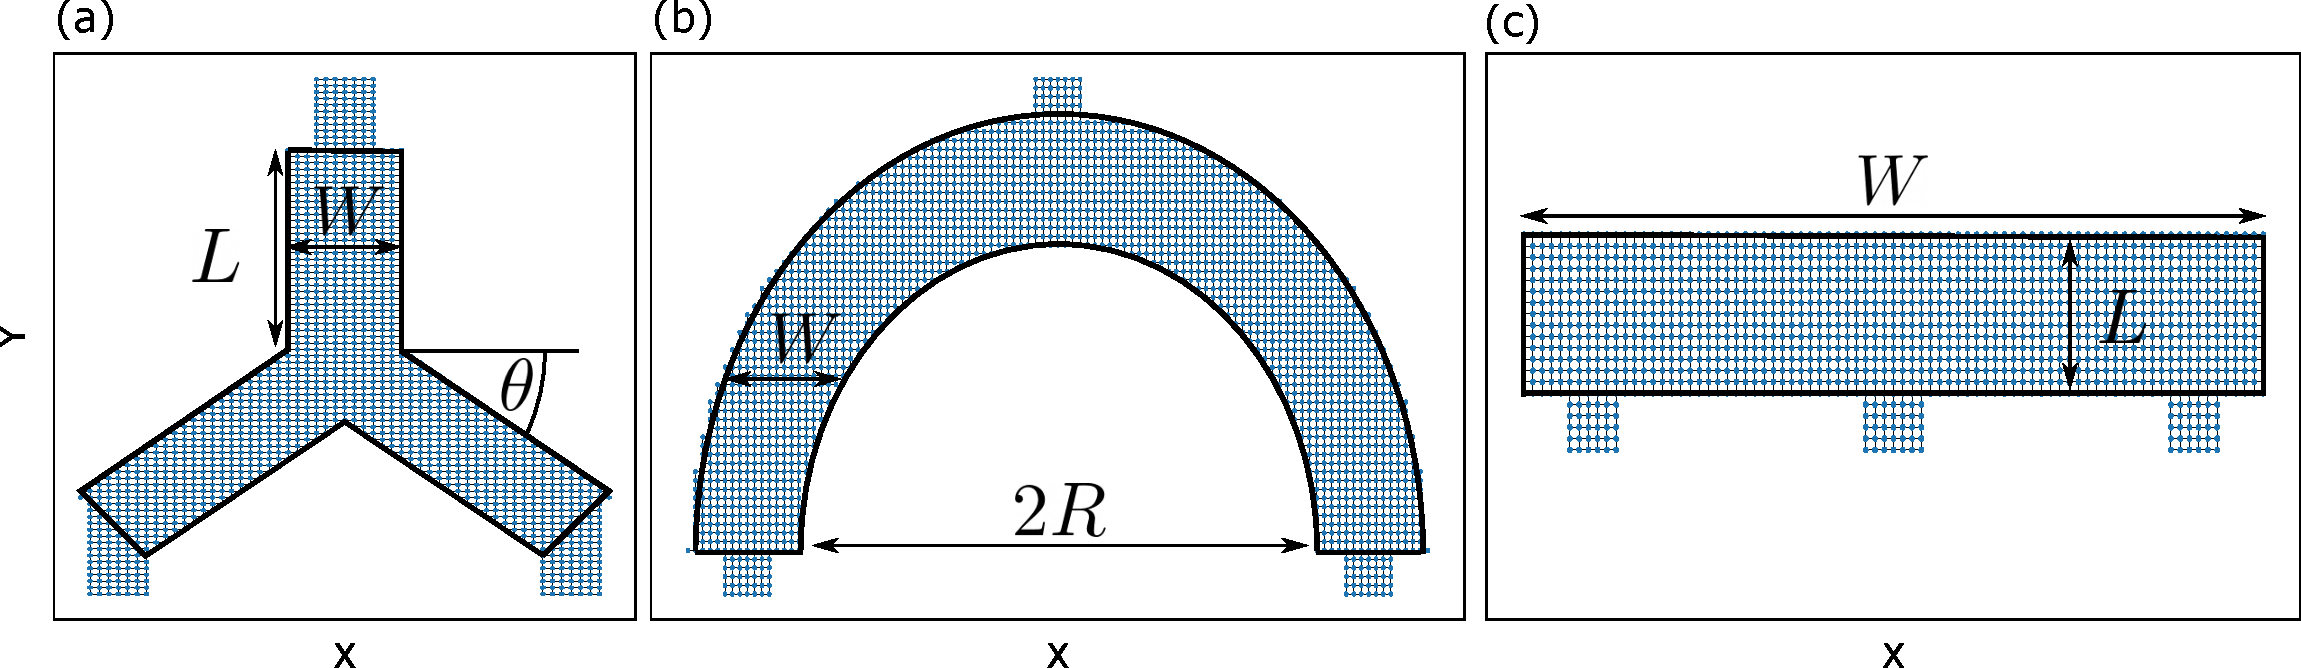
\includegraphics[width=0.7\linewidth]{figures/1d_cavities.pdf}
  \caption{Left: Kwant system of a half-ring shaped cavity. It is defined by the radius $R$ and the width $W$. Thiner rectangular segments represent the positions of the Majorana nanowires attached. Right: Lowest four eigenstates of the cavity with the nanowires fully depleted.}
  \label{fig:1d}
\end{figure}

The simplest cavity geometry to study MBS coupling is a stripe-like geometry.
The cavity eigenstates have a well-defines spatial structure, i.e. an integer number of nodes along the stripe axis.
\textit{We expect interference effects between the cavity state and MBS depending on their positions.}

We consider two quasi-one dimensional cavities:
In Fig. {fig:1d} (a) one can observe a rectangular stripe cavity with three Majorana nanowires attached. 
In Fig. \ref{fig:1d} (b) one can observe a half-ring stripe cavity with three Majorana nanowires attached in a fork-like geometry. 
\textit{The width of each cavity is fixed, and the length and nanowires position is changed.}

Mirror symmetry along the $x$-axis is imposed in the device.
Consequently, the phase shift is symmetric around $\pi$ for the central pairs as shown in Fig. \ref{fig:ring_results} (a).
\textit{However, the behaviour is oscillatory, non-trivial, and strongly depends on the geometry.}
The left right pair, similarly, has a nontrivial behaviour with a clearer periodicity than the other two pairs.
For each experiment, the phase is calibrated such that the coupling is maximum for the corresponding pair.

\begin{figure}[h!]
\centering
  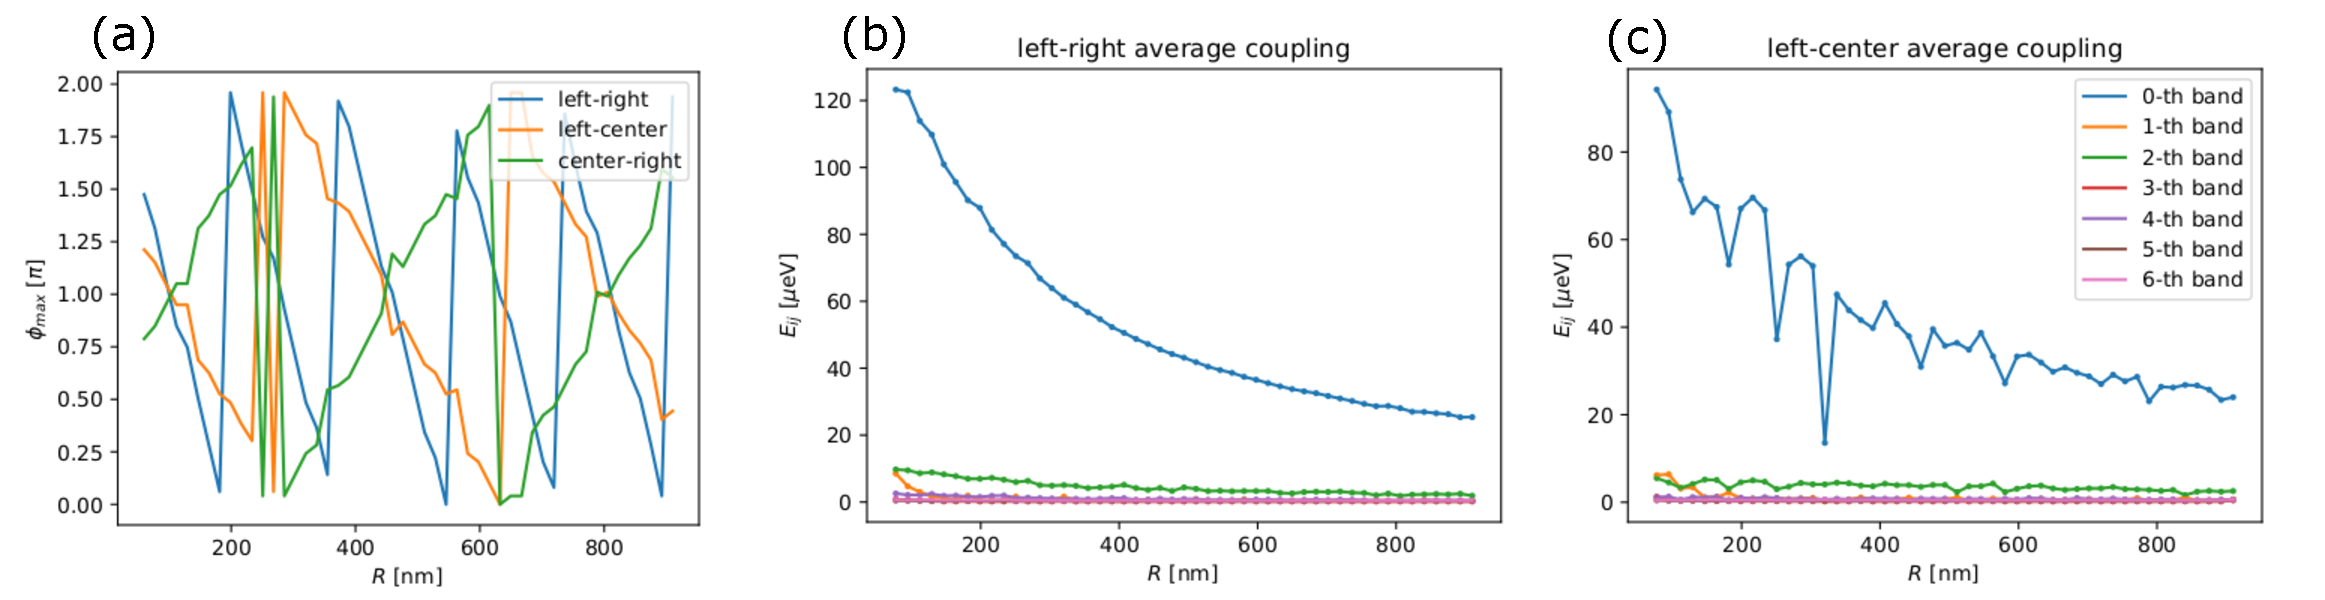
\includegraphics[width=\linewidth]{figures/ring_results.pdf}
  \caption{Results for half-ring cavity. (a) Phase shift $\phi_{max}$ vs. cavity radius $R$. (b) Coupling of left and right MBS pair. Colors show the band index of the nanowire. (c) Coupling of the left and central MBS pair. Remaining pair is not show since the results is the same as (b).}
  \label{fig:ring_results}
\end{figure}

Initially, we study the size dependence of a half-ring shaped cavity as depicted in Fig. \ref{fig:ring_results} (b)-(c).
For a small cavity, the MBS coupling behaves as in the quantum dot regime where the level spacing is large.
\textit{As the system size increase, the coupling spectra evolves from the short-junction limit to the long-junction limit.}
The number of states inside the gap increases, and the resonant peaks shrink.
For very large systems, the coupling decreases exponentially until it eventually vanishes for all pairs.

The coupling of different lead modes relies on momentum conservation.
If there are states with a similar momentum, then tunnel is allowed between the two structures.
In this case, the coupling is dominated by the lowest Majorana mode.
Therefore, in a quasi-one dimensional cavity there are few high-momentum channels that couple Majoranas in higher bands.

\subsection{Resonant trapping}

\begin{figure}[h!]
\centering
  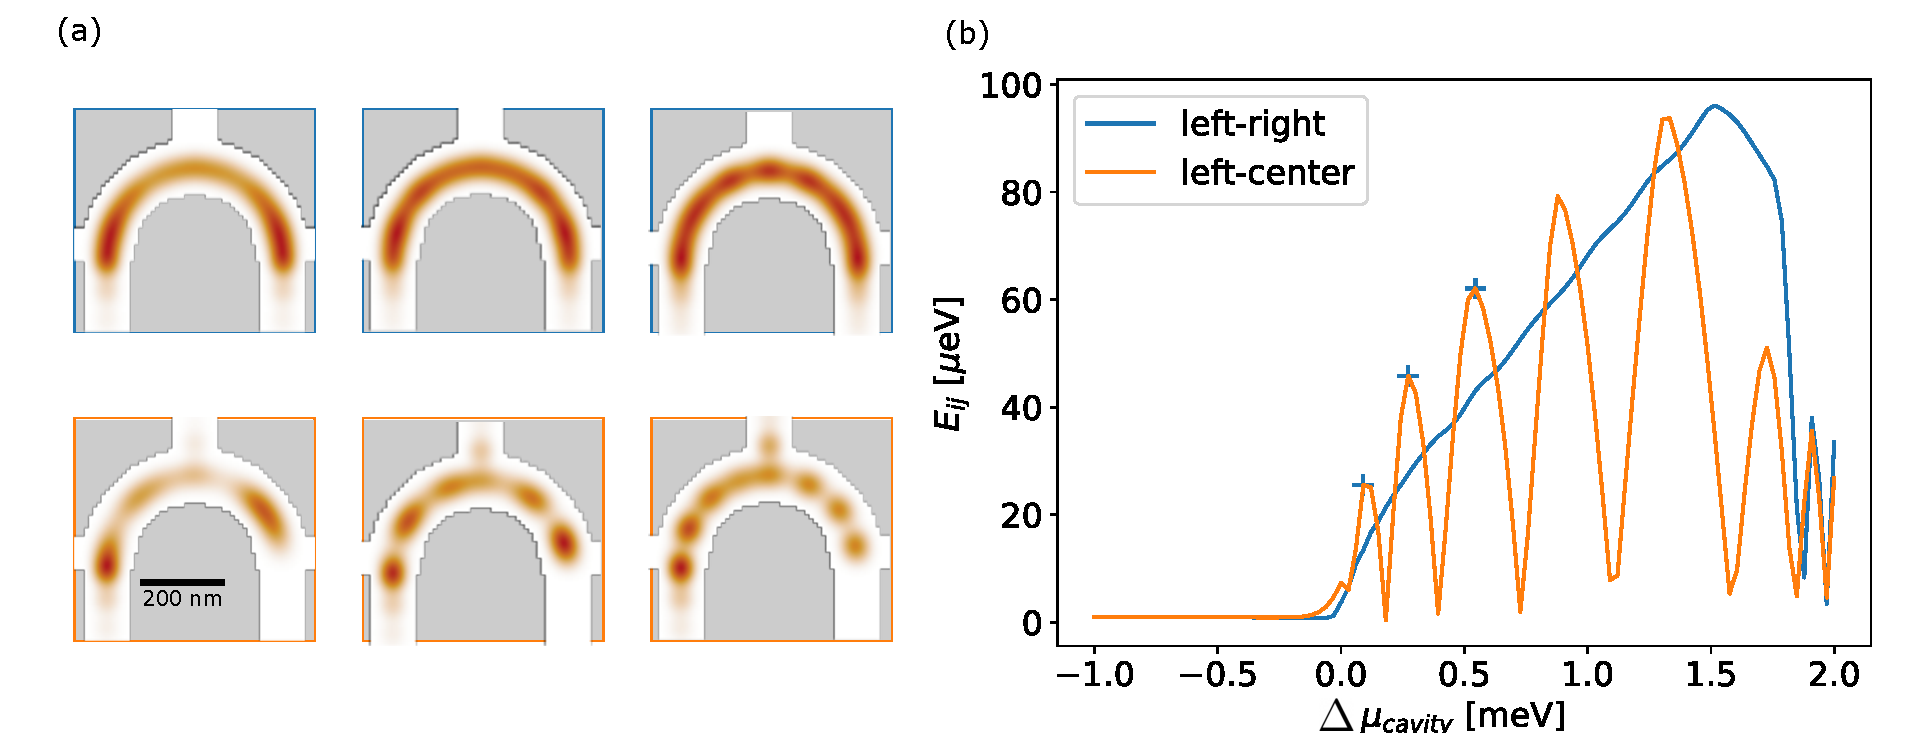
\includegraphics[width=\linewidth]{figures/resonant_trapping_ring.pdf}
  \caption{Spectra for a half-ring shaped cavity of width $W=110$ [nm] and radius $R=300$ [nm]. (a) Coupling of each MBS pair. Center-right pair is the same curve as left-center pair. Crosses indicate the positions at where the wavefunction (b) are taken. The color of the frame in (b) corresponds each MBS pair in (a).}
  \label{fig:resonant_trapping}
\end{figure}

Let us consider the half-ring cavity depicted in Fig. .When the left and right nanowires are close to the ends of the cavity, the MBS pair couple along a sequence of overlapping resonant states.
\textit{The cavity states interfere constructively and the coupling accumulates creating a single wide peak over the resonant region.}
This phenomena has been discussed in two-dimensional cavities when states along the convex border create a band of overlapping resonances with the lead states.
It is known as \textit{resonant trapping}.
This phenomena is reproduced in the rectangular-stripe geometry with nanowires attached at the far ends, yet the coupling is smaller.

\textit{This phenomena depends crucially on having the lead states around all of the cavity wavefunction.}
For the central pairs coupling, in contrast, a band of resonances cannot form since the cavity wavefunction is not fully enclosed.
When coupling the left and central MBS, the cavity region close to the right lead acts as a particle in a box with multiple individual levels that repel each other.
Therefore, we observe the two spectra shown in Fig. where one of them has a resonant band while in other the band is divided in individual resonances.

\section{Two dimensional cavities}

\begin{figure}[h!]
\centering
  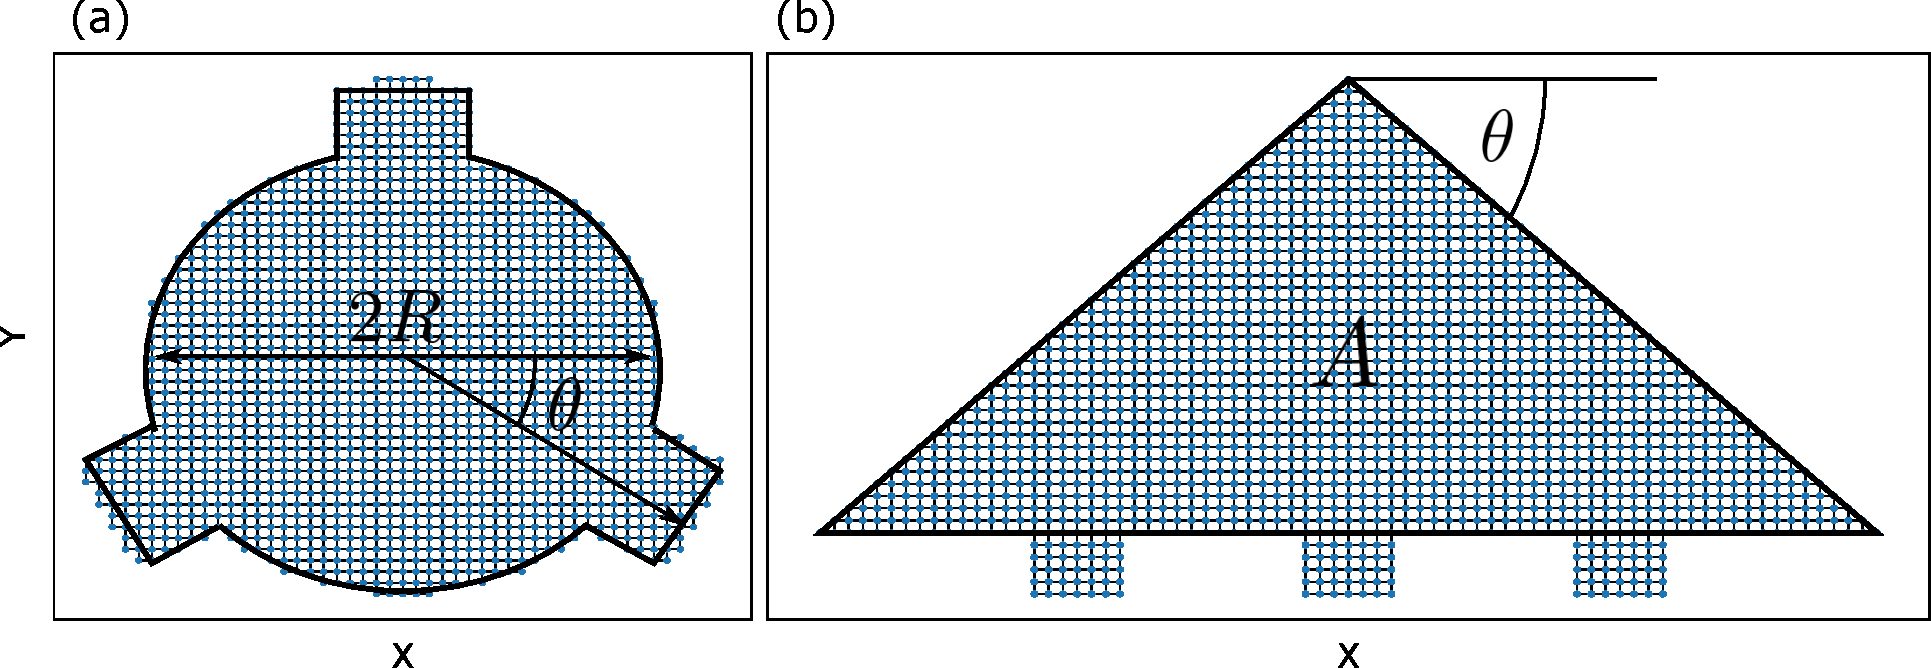
\includegraphics[width=0.7\linewidth]{figures/2d_cavities.pdf}
  \caption{Left: Kwant system of a half-ring shaped cavity. It is defined by the radius $R$ and the width $W$. Thiner rectangular segments represent the positions of the Majorana nanowires attached. Right: Lowest four eigenstates of the cavity with the nanowires fully depleted.}
  \label{fig:2d}
\end{figure}

In a ballistic cavity, the motion of the electrons is determined by the shape of the system.
From a semiclassical picture, trajectories connecting different leads contribute to the coupling of a given pair.
As the system size increases, however, the MBS coupling decreases as in the long-junction limit.
From the interplay of these two effect, we require \textit{the system size to be large enough to appreciate geometrical effects, but no large enough for the coupling to vanish.}

We study the MBS coupling of all pairs in three two-dimensional cavities. 
In Fig. one can observe a circular cavity defined by a radius $R$ with three nanowires symmetrically attached.
The left and right nanowires are attached at an angle $\theta$.
In Fig. one can observe a rectangular cavity defined by length $L$ and width $W$ with nanowires in a fork-like shape.
In Fig. one can observe a triangular cavity defined by an angle $\theta$ with nanowires attached in different configurations.
\textit{For the circular and rectangular cavity, the size is changed, while for the triangular cavity, the size is fixed and the angle is changed.}

The level spacing is smaller than in the quasi-one dimensional case, which means that the peaks will be narrower.
As before, the phase shift depends on each geometrical configuration, and it is optimised for each coupling experiment.
It is independent of the Majorana band.


\subsection{Circular cavity}

\begin{figure}[h!]
\centering
  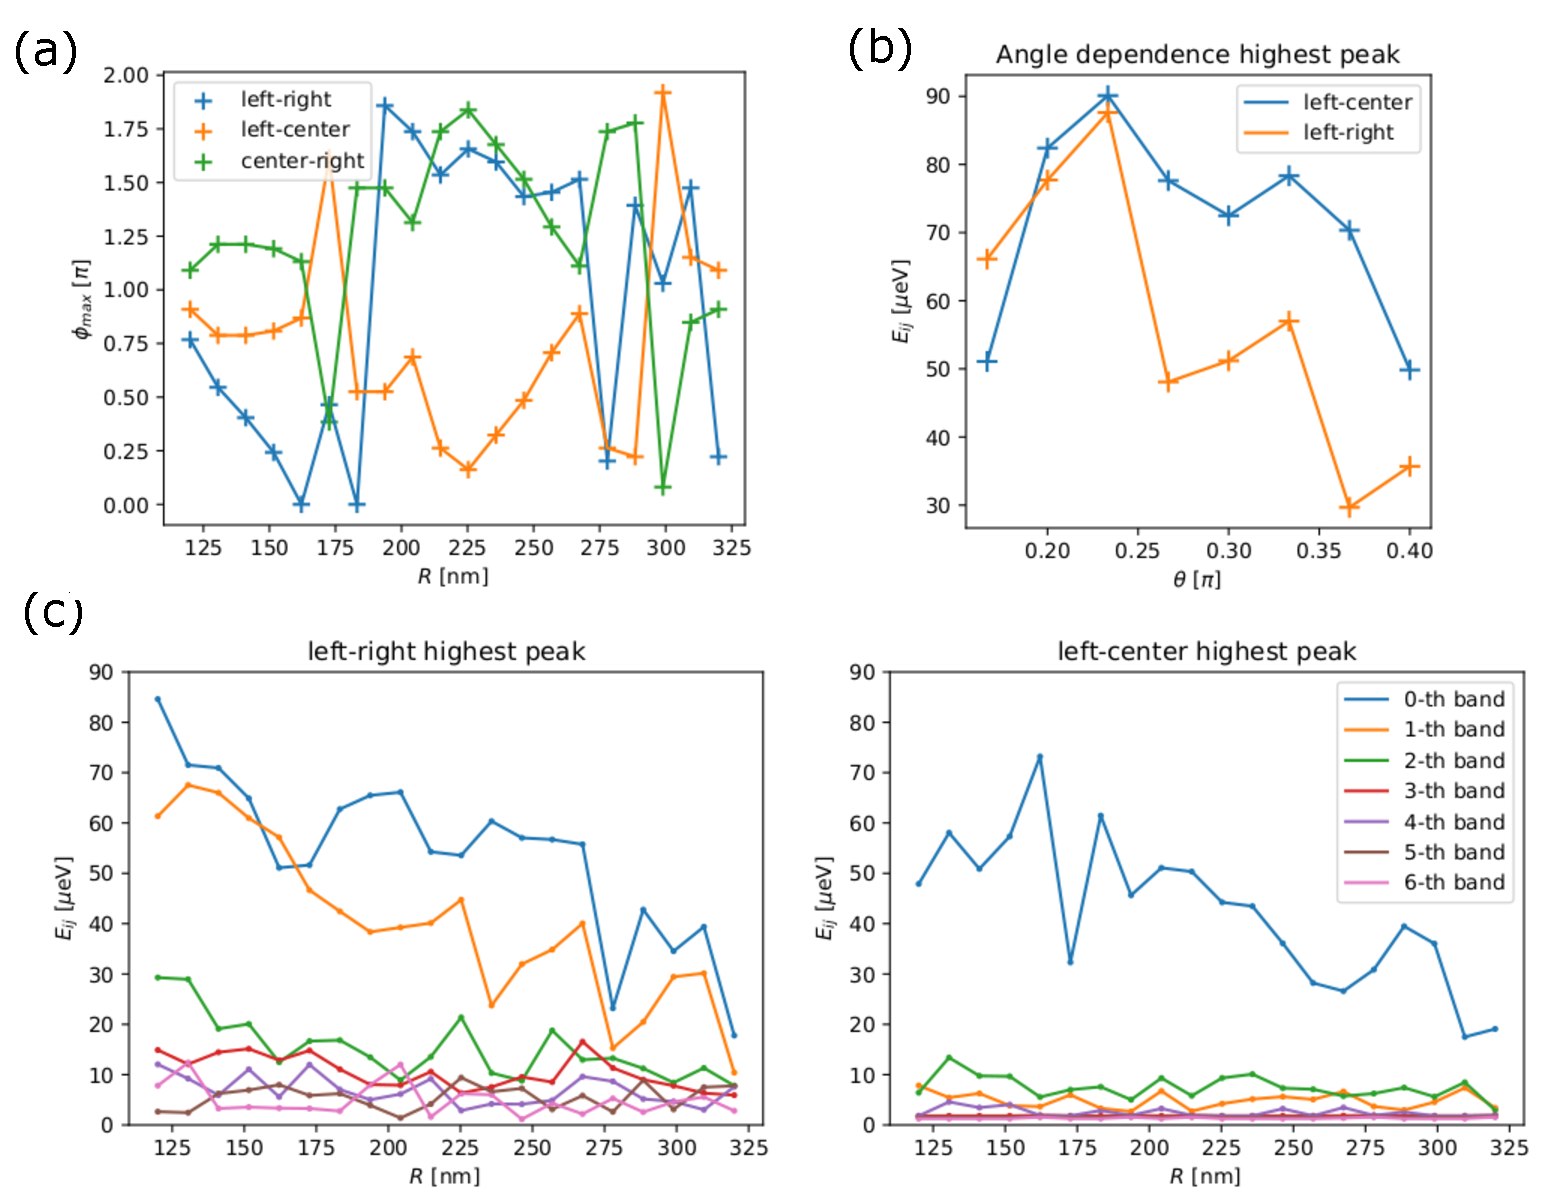
\includegraphics[width=0.8\linewidth]{figures/circle_results.pdf}
  \caption{Results for circular cavity. (a) Phase shift $\phi_{max}$ vs. circle radius $R$. (b) Coupling of left and right MBS pair. Colors show the band index of the nanowire. (c) Coupling of the left and central MBS pair. Remaining pair is not show since the results is the same as (b).}
  \label{fig:circle_results}
\end{figure}

Transport in a circular cavity has been extensively studied in semiconducting materials.
The contribution of each closed trajectory can be identified in the conductance.

The different Majorana sub bands couple non-trivially for each pair as is shown if Fig. \ref{fig:circle_results} (c)-(d).
The momentum profile of the states inside the cavity is similar for the lowest two band when the left and right MBS couple.
Consequently, it dominates over all the other bands.
On the other hand, for the central pairs, the coupling is significant only for the lowest sub band.
This implies that for the central MBS, the momentum distribution does not favour the coupling with the lateral MBS.

By changing the system size, one finds a transition between the short and long junction regimes.
For small cavities, $R=120$ [nm], the system behaves as a quantum dot with broad resonant peaks due to the large level spacing.
However, even in small systems, the coupling of the left and right MBS is larger than the one of the central pairs.
For large cavities, $R=300$ [nm], the resonant peaks become narrow and the coupling decreases.

In order to probe different trajectories, the angle of the left and right leads is changed and the result is shown if Fig. \ref{fig:circle_results} (b).
We choose a system with $R=200$ [nm] as an intermediate size where geometrical effects can be appreciated with a reasonable coupling.
By following the largest peak, one can observe a maximum coupling develop at $\theta = 0.23 \pi$.
In this case , the coupling of all pairs is dominated by the same level, which develops a high and narrow peak as the angle approaches this value.
As the angle increases further, there is a fast decay in the coupling for all pairs.

\section{Triangular cavity}

\textit{Given that in previous geometries, we have been able to modulate the coupling based on geometry, we pursue a similar approach in a triangular cavity as depicted in Fig. \ref{fig:2d} (b).}
By changing the angle of the diagonal sides of the cavity, we expect to modulate the coupling such it is enhanced for a given pair.
The area of the triangle is fixed, and consequently the length of the lateral sides will change for every angle.
On this setup, the relative position of the nanowires is fixed to lie at the center of the diagonal sides.

\subsection{Angular dependence}

\begin{figure}[h!]
\centering
  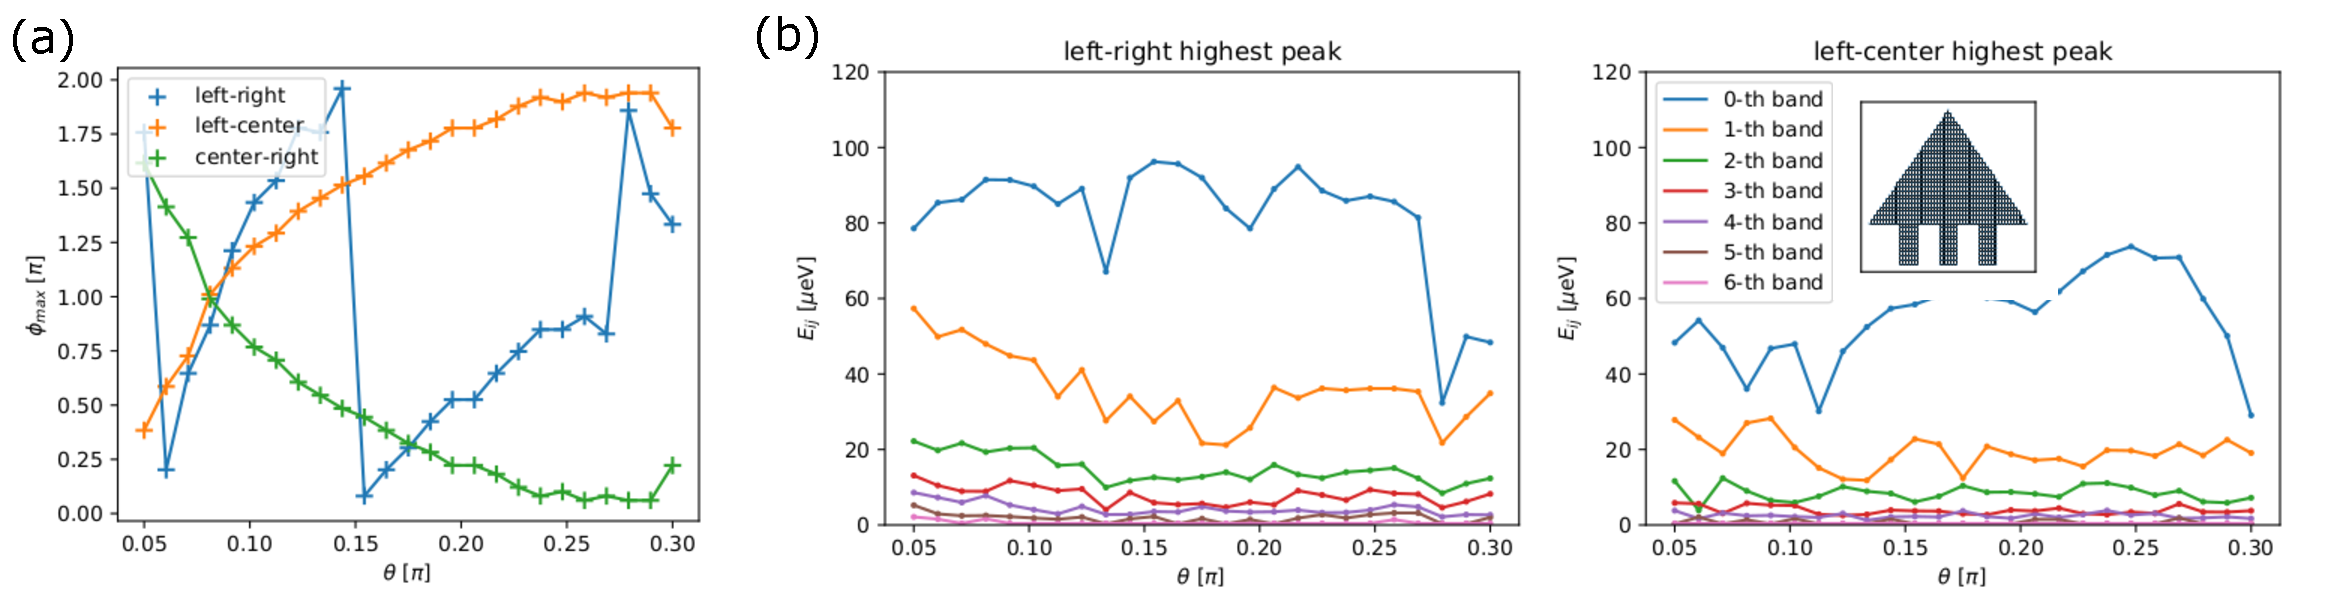
\includegraphics[width=0.8\linewidth]{figures/triangle_one_side_results.pdf}
  \caption{Results for circular cavity. (a) Phase shift $\phi_{max}$ vs. circle radius $R$. (b) Coupling of left and right MBS pair. Colors show the band index of the nanowire. (c) Coupling of the left and central MBS pair. Remaining pair is not show since the results is the same as (b).}
  \label{fig:average_ring_coupling}
\end{figure}

The left and right MBS mean coupling remains roughly the same when the angle of the diagonal sides changes.
However the coupling mechanism is different for small and large angles.
For small angles, the triangular cavity resembles a cutted rectangular strip where the wavefunction weight is concentrated in the central part of the cavity.
Therefore, resonant trapping couples the MBS over a range of cavity levels.
As the angle increases, the highest levels of the resonant band will decouple into individual peaks.
For large angles, the coupling will be mediated by individual resonances.

For the central MBS pairs, the mean coupling increases with the angle.
For angles around $\theta=\pi/4$ these pairs reach a maximum coupling.
As before, most of the coupling will be carried by the lowest Majorana band.

\subsection{Lead position dependence}

\begin{figure}[h!]
\centering
  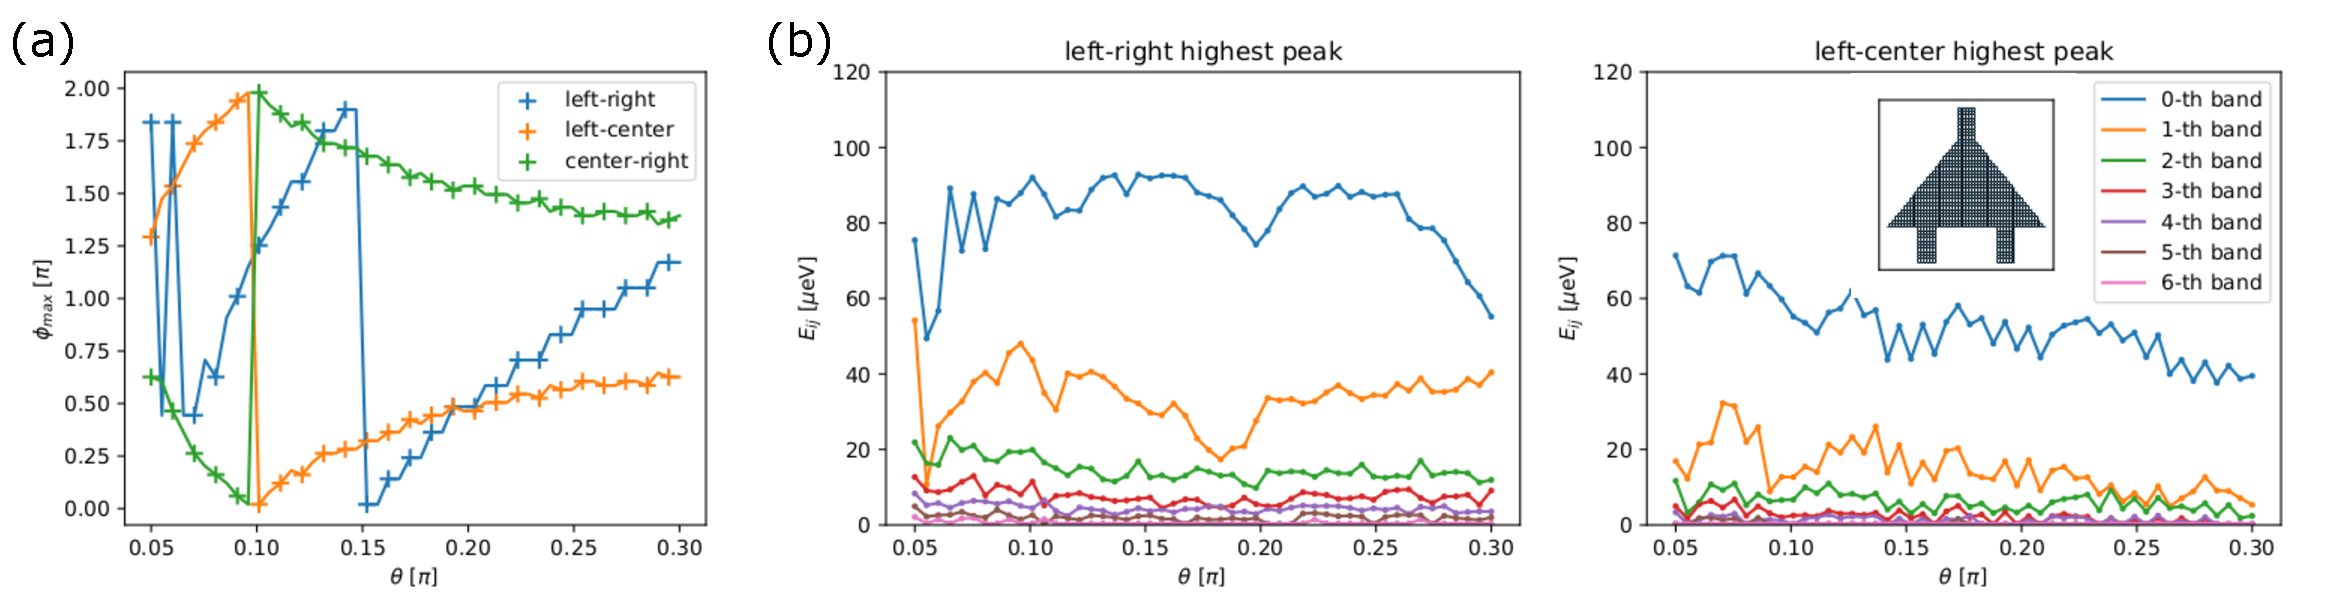
\includegraphics[width=0.8\linewidth]{figures/triangle_two_side_results.pdf}
  \caption{Results for circular cavity. (a) Phase shift $\phi_{max}$ vs. circle radius $R$. (b) Coupling of left and right MBS pair. Colors show the band index of the nanowire. (c) Coupling of the left and central MBS pair. Remaining pair is not show since the results is the same as (b).}
  \label{fig:average_ring_coupling}
\end{figure}

The position of the central lead inverts the angle dependence of the central MBS pairs coupling.
As can be observed in Fig. (c), the coupling decreases with angle, yet it remains at a comparable value with respect to the case with the lead in the lower side.

Similarly, the position of the left and right leads can be taken to the opposite side.
In such case, we have found that the coupling decreases by approximately $1/2$.
Nevertheless, the coupling of the higher momentum bands becomes much larger than in all previous cases.

\section{Summary}

Overall, all the geometries can be classified according to the mean coupling and the mean level spacing as in Fig. \ref{fig:comparison}. 
The quasi-one dimensional geometries show a much larger coupling and level spacing.
This is reasonable because of the system size and dimensionality.
For two-dimensional systems, on the other hand, it is not trivial what the geometry effect would be.
One can observe that the circular geometry has the smaller level spacing and mean coupling.
The two triangular cavities are close to each other.
The difference between them is induced by the position of the central lead.

\begin{figure}[h!]
\centering
  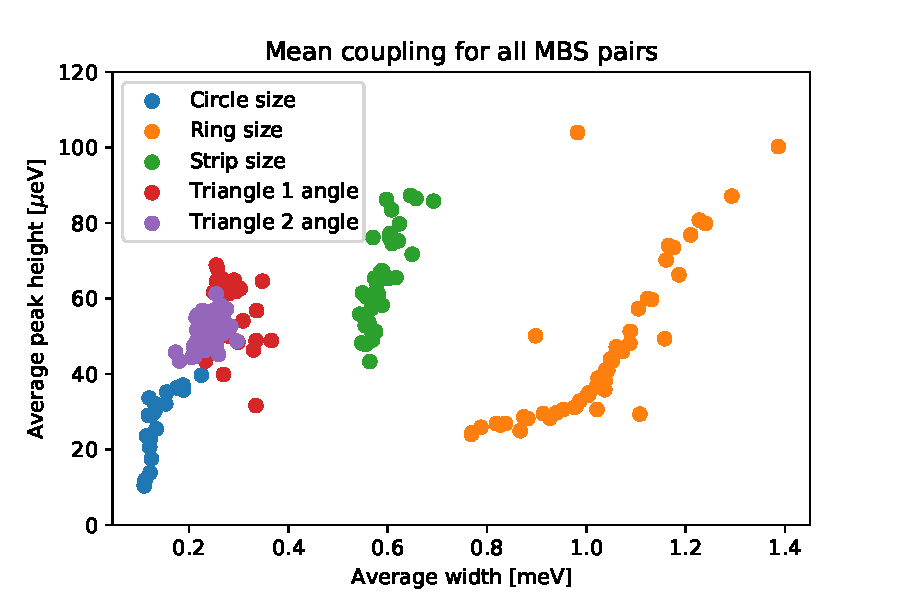
\includegraphics[width=0.8\linewidth]{figures/comparison.pdf}
  \caption{}
  \label{fig:comparison}
\end{figure}




